\begin{Definition}{facets}
  Let $\cell\subset \R^d$ be a polyhedron. We call the lower
  dimensional polyhedra constituting its boundary \define{facet}s. A
  facet of dimension zero is called \define{vertex}, of dimension one
  \define{edge}, and a facet of codimension one is called a
  \define{face}.
\end{Definition}

\begin{Definition}{mesh}
  A \define{mesh} $\mesh$ is a nonoverlapping subdivision of the
  domain $\domain$ into polyhedral \define{cell}s denoted by $\cell$,
  for instance simplices, quadrilaterals, or hexahedra. The
  faces of a cell are denoted by $\face$, the
  vertices by $\vertex$. Cells are typically considered open sets.

  A mesh $\mesh$ is called regular, if each face
  $\face \subset \d\cell$ of the cell $\cell\in\mesh$ is either a
  face of another cell $\cell\prime$, that is,
  $\overline{\face} = \overline{\cell} \cap \overline{\cell\prime}$,
  or a subset of $\d\domain$.
\end{Definition}

\begin{remark}
  For this introduction, we will assume that indeed $\domain$ is the
  union of mesh cells, which means, that its boundary consists of a
  finite union of planar faces. The more general case of a mesh
  approximating the domain will be deferred to later discussion.
\end{remark}

\begin{Definition}{finite-element}
  With a mesh cell $\cell$, we associate a finite dimensional
  \define{shape function} space $\shapespace(\cell)$ of dimension
  $n_\cell$. The term \define{node functional} denotes linear
  functionals on this space.

  A set of node functionals $\{\nodal_\cell^i\}_{i=1,\dots,n_\cell}$ is called
  \define{unisolvent} on $\shapespace(\cell)$ if for any vector
  $\vu = (u_1,\dots,u_{n_\cell})^T$ there exists a unique
  $u\in \shapespace(\cell)$ such that
  \begin{gather}
    \nodal_\cell^i(u) = \vu_i,\quad i=1,\dots,n_\cell.
  \end{gather}

  A \define{finite element} is a set of shape function spaces
  $\shapespace(\cell)$ for all $\cell\in\mesh$ together with
  unisolvent set of node functionals.
\end{Definition}

\begin{Notation}{dofs}
  If the node functionals $\nodal^i$ are unisolvent on
  $\shapespace(\cell)$, then, there is a basis $\{p_k\}$ of $\shapespace(\cell)$
  such that
  \begin{gather}
    \nodal^i(p_k) = \delta_{ik}.
  \end{gather}
  We refer to $\{p_k\}$ as \define{shape function basis} and use the
  term \define{degrees of freedom} for both the node functionals and
  the basis functions.
\end{Notation}

\begin{Definition}{node-topology}
  Node functionals can be associated with the cell $\cell$ or with one
  of its lower dimensional boundary facets. We call this association
  the \define{topology} of the finite element.
\end{Definition}

\begin{Definition}{fe-space}
  The \define{finite element space} on the mesh $\mesh$, denoted by
  $V_\mesh$ is a subset of the concatenation of all shape function
  spaces,
  \begin{gather}
    V_\mesh \subset \bigl\{ f\in L^2(\domain) \big|
    f_{\cell} \in \shapespace(\cell) \bigr\}.
  \end{gather}
  The \define{degrees of freedom} of $V_\mesh$ are the union of all
  node functionals, where we identify node functionals associated to
  boundary facets among all cells sharing this facet. The resulting
  dimension is
  \begin{gather}
    n = \dim V_\mesh \le \sum n_\cell.
  \end{gather}
\end{Definition}

\begin{figure}[tp]
  \begin{center}
    \includegraphics[width=.5\textwidth]{graph/concatenation.tikz}
  \end{center}
  \caption{Identification of node functionals. The node functionals on
    shared edges (separated for presentation purposes) are
    distinguished locally as belonging to their respective cells, but
    identical global indices are assigned to all nodes in a single
    circle. Thus, all associated shape functions obtain the same
    coefficient in the global basis representation of a finite element
    function $u$.}
  \label{fig:nodes-identification}
\end{figure}

\begin{Notation}{global-local}
  When we enumerate the degrees of freedom of $V_\mesh$, we obtain a
  global numbering of degrees of freedom $\nodal^i$ with
  $i=1,\dots,n$. For each mesh cell, we have a local numbering
  $\nodal_\cell^j$ with $j=1,\dots,n$. By construction of the finite
  element space, there is a unique $i$, such that
  $\nodal_\cell^j(f) = \nodal^i(f)$ for all cells $\cell$ and local
  indices $j$. The converse is not true due to the identification
  process.
\end{Notation}

\begin{Definition}{local-global}
  We refer to the mapping between $\nodal^i$ and $\nodal_\cell^j$ as
  the mapping between global and local indices
  \begin{gather}
    \iota: (\cell, j) \mapsto i.
  \end{gather}
  It induces a
  ``natural'' basis $\{v_i\}$ of $V_\mesh$ by
  \begin{gather}
    v_{i|\cell} = p_{\cell,j},
  \end{gather}
  where $\{p_{\cell,j}\}$ is the shape function basis on $\cell$. For
  each $\nodal^i$, we define $\mesh(\nodal^i)$ as the set of cells
  $\cell$ sharing the node functional $\nodal^i$, and
  \begin{gather}
    \domain\left(\nodal^i\right) = \bigcup_{\cell\in \mesh(\nodal^i)} \cell.
  \end{gather}
\end{Definition}

\begin{Lemma}{fe-support}
  The support of the basis function $v_i\in V_\mesh$ is
  \begin{gather*}
    \operatorname{supp}(v_i) \subset \domain\left(\nodal^i\right).
  \end{gather*}
\end{Lemma}

\begin{Lemma}{mesh-continuity}
  Let $\mesh$ be a subdivision of $\domain$, and let $u$ be a function
  on $\domain$, such that $u_{|\cell} \in C^1(\cell)$. Then,
  \begin{gather}
    u\in H^1(\domain)
    \quad \Longleftrightarrow\quad
    u\in C(\overline\domain).
  \end{gather}
\end{Lemma}

\begin{Lemma}{nodal-continuity}
  We have $V_\mesh\subset C(\overline{\domain})$ if and only if for
  every facet $F$ of dimension $d_F < d$ there holds that
  \begin{enumerate}
  \item the traces of the spaces $\shapespace(\cell)$ on $F$ coincide
    for all cells $\cell$ having $F$ as a facet,
  \item The node functionals associated to the facet are unisolvent on
    this trace space.
  \end{enumerate}
\end{Lemma}

%%%%%%%%%%%%%%%%%%%%%%%%%%%%%%%%%%%%%%%%%%%%%%%%%%%%%%%%%%%%%%%%%%%%%%
%%%%%%%%%%%%%%%%%%%%%%%%%%%%%%%%%%%%%%%%%%%%%%%%%%%%%%%%%%%%%%%%%%%%%%
\subsection{Shape function spaces on simplices}
%%%%%%%%%%%%%%%%%%%%%%%%%%%%%%%%%%%%%%%%%%%%%%%%%%%%%%%%%%%%%%%%%%%%%%
%%%%%%%%%%%%%%%%%%%%%%%%%%%%%%%%%%%%%%%%%%%%%%%%%%%%%%%%%%%%%%%%%%%%%%

\begin{Definition}{barycentric-coordinates}
  A simplex $\cell\in \R^d$ with vertices $\vertex_0,\dots,\vertex_d$
  is described by a set of $d+1$ \define{barycentric coordinates}
  $\vlambda = (\lambda_0,\dots,\lambda_d)^T$ such that
  \begin{xalignat}2
    0\le\lambda_i &\le 1& i&=0,\dots,d;\\
    \lambda_i(\vertex_j) &= \delta_{ij}& i,j&=0,\dots,d\\
    \sum \lambda_i(\vx) &= 1,
  \end{xalignat}
  and there holds
  \begin{gather}
    T = \Bigl\{x\in\R^d \Big| x = \sum \vertex_k\lambda_k \Bigr\}.
  \end{gather}
\end{Definition}

\begin{Lemma}{barycentric-affine}
  There is a matrix $B_T\in \R^{d+1\times d}$ and a vector
  $b_T\in\R^{d+1}$, such that
  \begin{gather}
    \vlambda = B_T\vx + b_T.
  \end{gather}
\end{Lemma}

\begin{Corollary}{barycentric-interpolation}
  The barycentric coordinates $\lambda_0,\dots,\lambda_d$ are the
  linear Lagrange interpolating functions for the points
  $\vertex_0,\dots,\vertex_d$. In particular, $\lambda_k \equiv 0$ on
  the facet not containing $\vertex_k$.
\end{Corollary}

\begin{example}
  We can use barycentric coordinates to define interpolating polynomials on
  simplicial meshes easily, as in
  Table~\ref{tab:barycentric-shapes}.
  \begin{table}[tp]
    \centering
    \begin{tabular}{|c|l|}
      \hline Degrees of freedom
      & Shape functions \\\hline
      \adjustbox{valign=center,margin=3pt}{\includegraphics[width=2cm]{mixed/fig/p1-p.tikz}}
      &
        {\begin{minipage}[b]{6cm}
          \begin{gather*}
            \phi_i = \lambda_i,
            \quad i=0,1,2
          \end{gather*}
        \end{minipage}}
      \\\hline
      \adjustbox{valign=center,margin=3pt}{\includegraphics[width=2cm]{mixed/fig/p2-p.tikz}}
      &
        {\begin{minipage}[b]{6cm}
          \begin{xalignat*}2
            \phi_{ii} &= 2\lambda_i^2 - \lambda_i,
            &i&=0,1,2\\
            \phi_{ij} &= 4\lambda_i\lambda_j
            &j&\neq i
          \end{xalignat*}
        \end{minipage}}
        \\\hline
      \adjustbox{valign=center,margin=3pt}{\includegraphics[width=2cm]{mixed/fig/p3-p.tikz}}
      &
        {\begin{minipage}[b]{6cm}
          \begin{xalignat*}2
          \phi_{iii} &= \tfrac12 \lambda_i(3\lambda_i-1)(3\lambda_i-2)
          &i&=0,1,2\\
          \phi_{ij} &= \tfrac92\lambda_i\lambda_j(3\lambda_j-1)
          &j&\neq i\\
          \phi_0 &= 27\lambda_0\lambda_1\lambda_2
        \end{xalignat*}
        \end{minipage}}
        \\\hline
    \end{tabular}
    \caption{Degrees of freedom and shape functions of simplicial elements
      in terms of barycentric coordinates}
    \label{tab:barycentric-shapes}
  \end{table}
\end{example}

\begin{remark}
  The functions $\lambda_i(x)$ are the shape functions of the linear
  $P_1$ element on $T$. They allow us to define basis functions on the
  cell $T$ without use of a reference element $\widehat T$.

  Note that $\lambda_i\equiv 0$ on the face opposite to the
  vertex $x_i$.
\end{remark}

%%%%%%%%%%%%%%%%%%%%%%%%%%%%%%%%%%%%%%%%%%%%%%%%%%%%%%%%%%%%%%%%%%%%%%
%%%%%%%%%%%%%%%%%%%%%%%%%%%%%%%%%%%%%%%%%%%%%%%%%%%%%%%%%%%%%%%%%%%%%%
\subsection{Shape functions on tensor product cells}
%%%%%%%%%%%%%%%%%%%%%%%%%%%%%%%%%%%%%%%%%%%%%%%%%%%%%%%%%%%%%%%%%%%%%%
%%%%%%%%%%%%%%%%%%%%%%%%%%%%%%%%%%%%%%%%%%%%%%%%%%%%%%%%%%%%%%%%%%%%%%

\begin{Definition}{tensor-product-polynomials}
  The space of \define{tensor product polynomials} of degree $k$ in
  $d$ dimensions, denoted as $\Q_k$ consists of polynomials of degree
  up to $k$ in each variable. Given a basis for one-dimensional
  polynomials $\{p_i\}_{i=0,\dots,k}$, a natural basis for $\Q_k$ is
  the \define{tensor product basis}
  \begin{gather}
    \label{eq:fem-intro:1}
    p_{i_1,\dots,i_d}(\vx)
    = p_{i_1}\otimes \dots\otimes p_{i_d}
    = \prod_{k=1}^d p_{i_k}(x_k).
  \end{gather}
\end{Definition}

\begin{remark}
  Note that the basis functions of $\Q_k$ can be denoted as products
  of univariate polynomials, but that general polynomials in this
  space as linear combinations of these basis functions do not have
  this structure.
\end{remark}

\begin{Lemma}{tensor-product-node-functionals}
  Let $\{\nodal_j\}$ be a set of one-dimensional node functionals dual
  to the one-dimensional basis $\{p_i\}$ such that
  \begin{gather}
    \nodal_j(p_i) = \delta_{ij}.
  \end{gather}
  Then, a dual basis for $\{p_{i_1,\dots,i_d}\}$ is obtained by
  defining on the tensor product basis of $\Q_k$
  \begin{gather}
    \label{eq:fem-intro:2}
    \nodal_{j_1,\dots,j_d}(p_{i_1,\dots,i_d})
    = \nodal_{j_1} \otimes \dots\otimes \nodal_{j_d}(p_{i_1}\otimes\dots\otimes p_{i_d})
    = \prod_{k=1}^d \nodal_{j_k}(p_{i_k}).
  \end{gather}
\end{Lemma}

\begin{proof}
  It is a theorem in linear algebra, that a linear functional on a
  vector space is uniquely defined by its values on a basis of the
  space. Thus,~\eqref{eq:fem-intro:2} uniquely defines the node
  functionals $\nodal_{j_1,\dots,j_d}$. The duality property follows
  from the fact that
  \begin{gather*}
    \nodal_{j_1,\dots,j_d}(p_{i_1,\dots,i_d}) = \prod_{k=1}^d \delta_{i_k,j_k},
  \end{gather*}
  which is one if and only if all index pairs match and zero in all
  other cases.
\end{proof}

\begin{example}
  Let a basis $\{p_i\}$ of the univariate space $\P_k$ be defined by
  Lagrange interpolation in $k+1$ points $t_j \in [0,1]$. A basis of
  the $d$-dimensional space $\Q_k$ is then obtained by all possible
  products
  \begin{gather*}
    p_{i_1,\dots,i_d}(\vx) = \prod_{k=1}^d p_{i_k}(x_k).
  \end{gather*}
  The node functionals following the construction above are obtained by
  \begin{gather*}
    \nodal_{j_1,\dots,j_d}(p_{i_1,\dots,i_d}) = \prod_{k=1}^d p_{i_k}(x_{j_k}).
  \end{gather*}
  Finally, we have to convert the term on the right into an
  expression, which can be applied to any polynomial in $\Q_k$. To
  this end, we observe that
  \begin{gather*}
    \prod_{k=1}^d p_{i_k}(x_{j_k}) = p_{i_1,\dots,i_d}(x_{j_1},\dots,x_{j_d}).
  \end{gather*}
  Therefore, we conclude that the tensor product node functionals
  resulting from this construction are
  \begin{gather*}
    \nodal_{j_1,\dots,j_d}(p) = p(x_{j_1},\dots,x_{j_d}).
  \end{gather*}
\end{example}

\begin{Example*}{q2}{The space $\Q_2$}
    \begin{center}
    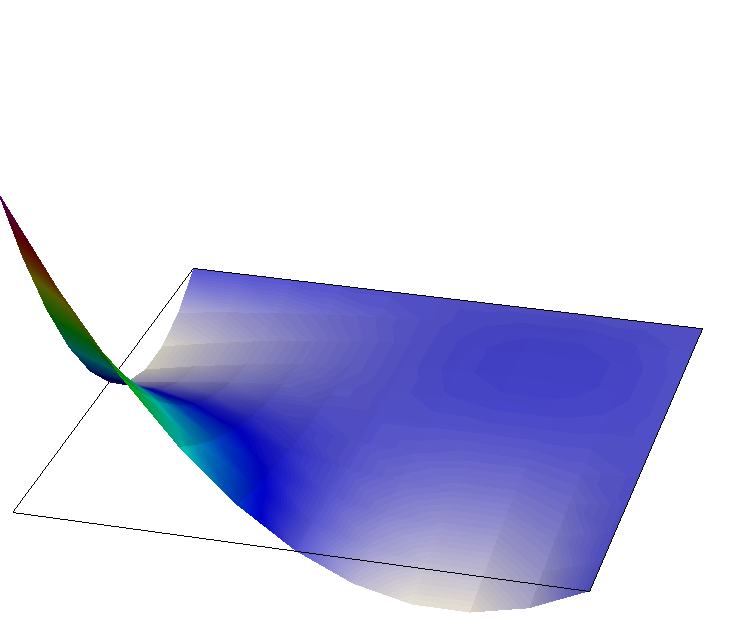
\includegraphics[width=.3\textwidth]{graph/shape0}
    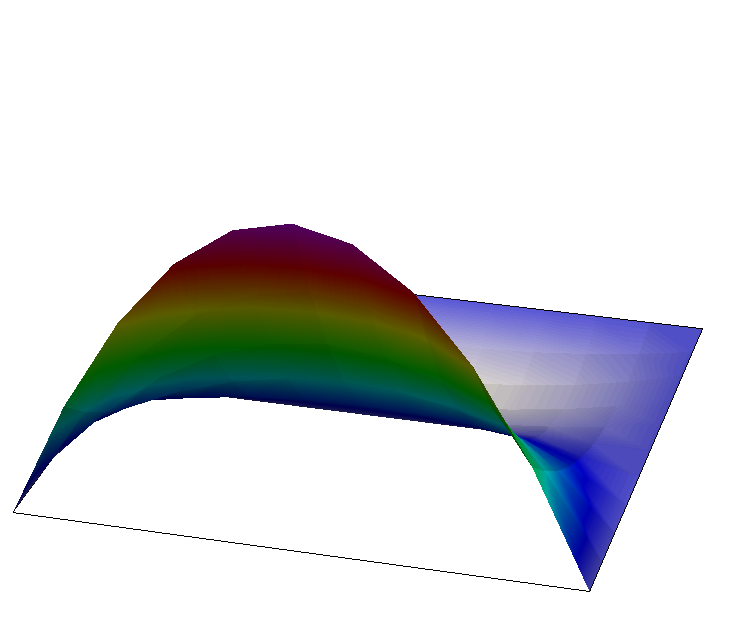
\includegraphics[width=.3\textwidth]{graph/shape1}
    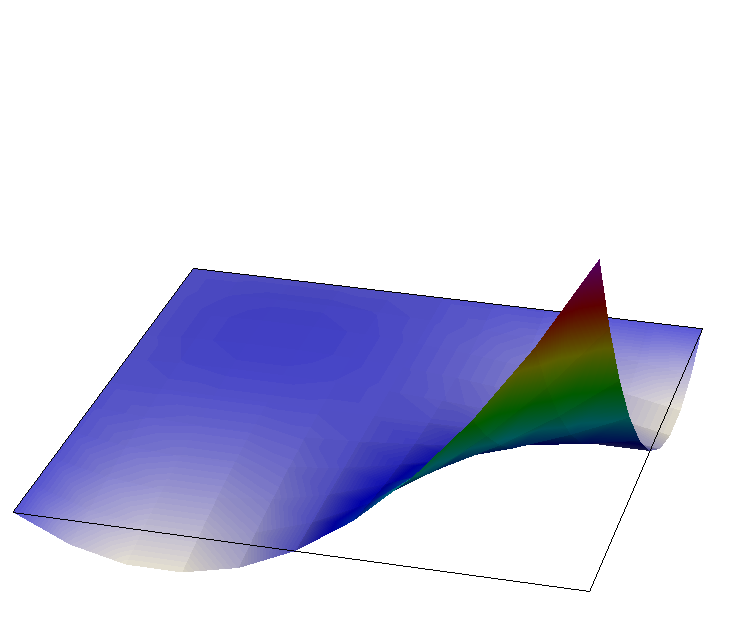
\includegraphics[width=.3\textwidth]{graph/shape2}

    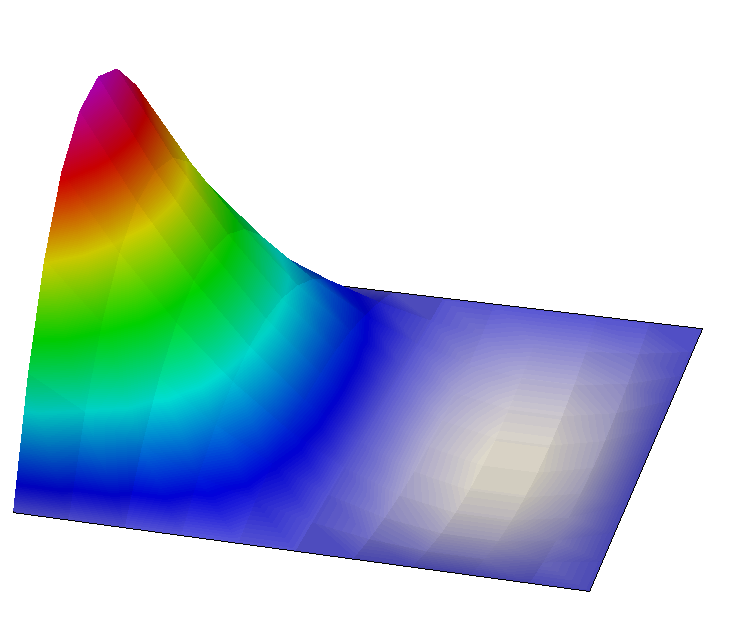
\includegraphics[width=.3\textwidth]{graph/shape3}
    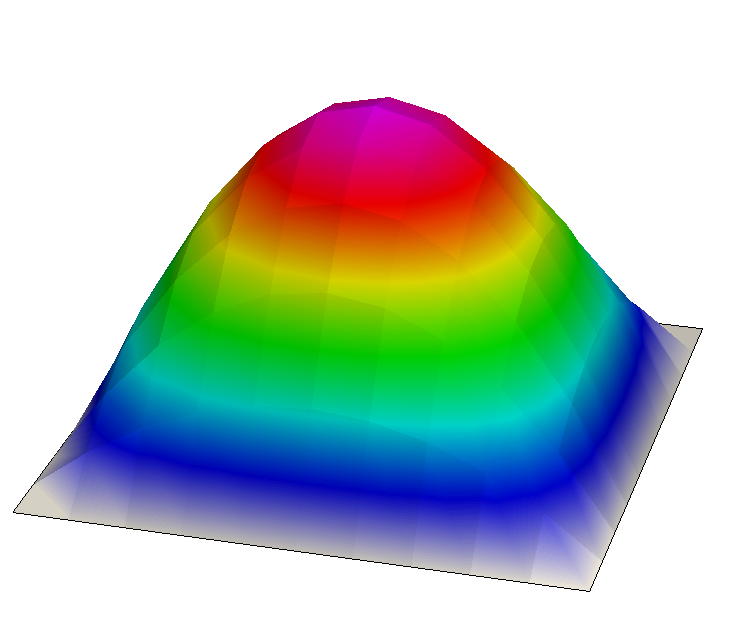
\includegraphics[width=.3\textwidth]{graph/shape4}
    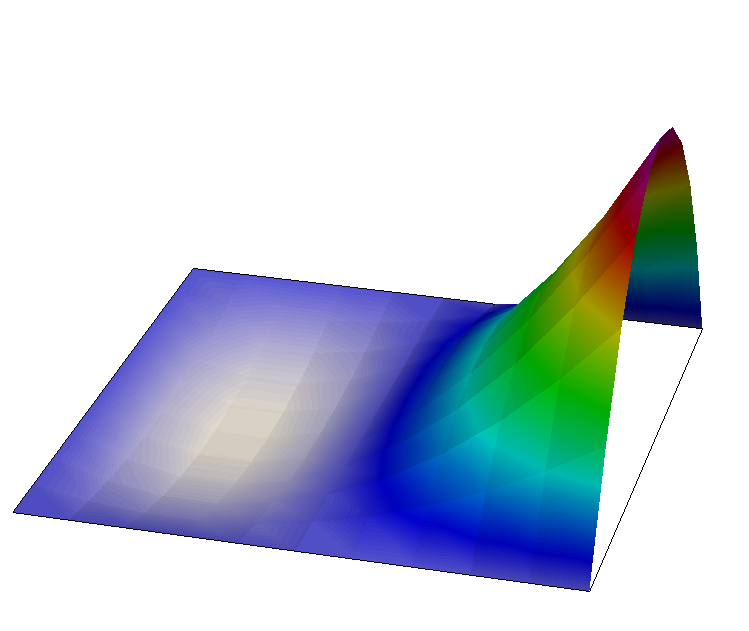
\includegraphics[width=.3\textwidth]{graph/shape5}

    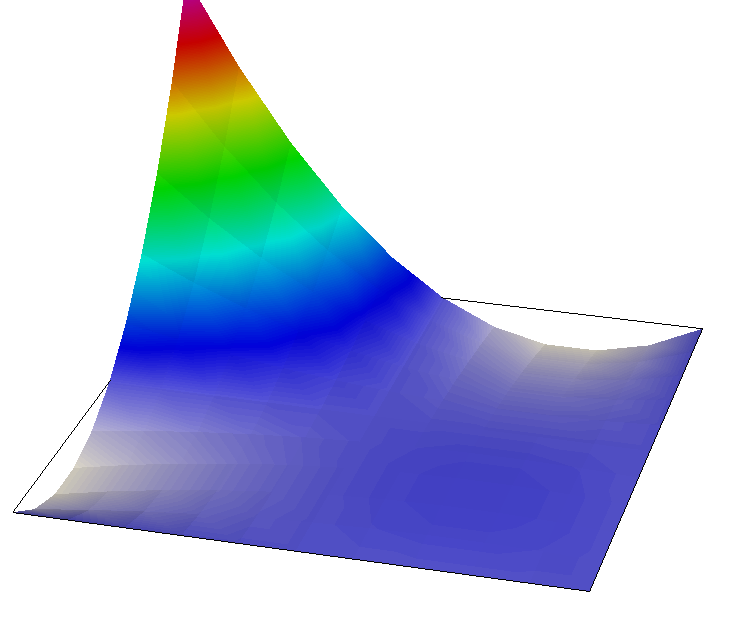
\includegraphics[width=.3\textwidth]{graph/shape6}
    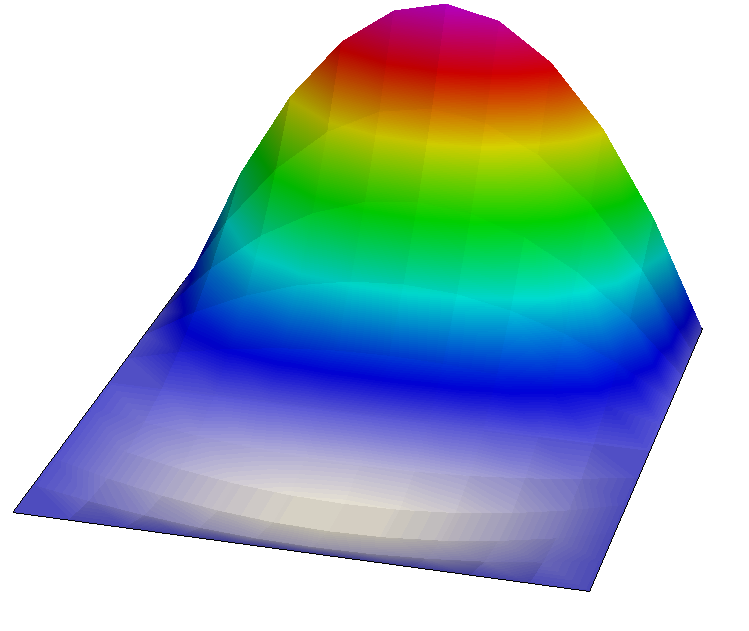
\includegraphics[width=.3\textwidth]{graph/shape7}
    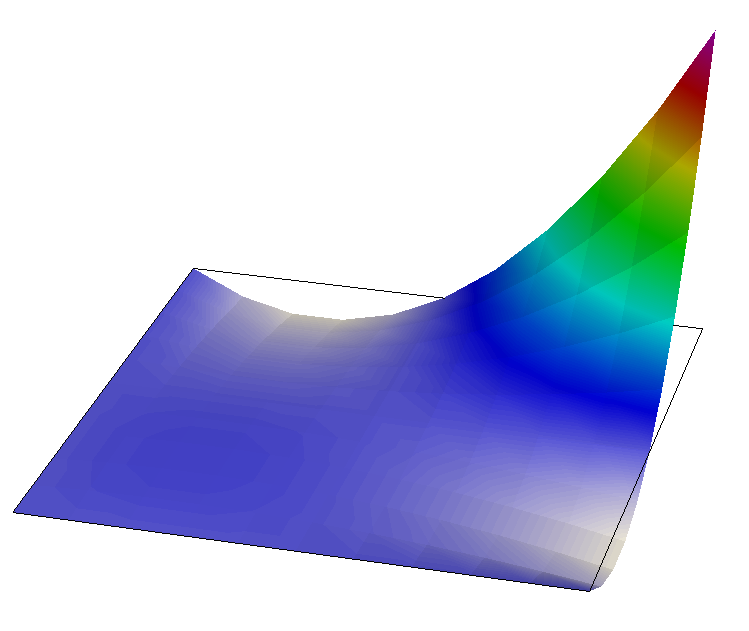
\includegraphics[width=.3\textwidth]{graph/shape8}
  \end{center}
\end{Example*}


\begin{Lemma}{tensor-product-trace}
  The trace of the $d$-dimensional tensor product polynomial space
  $\Q_k$ on the $\delta$-dimensional facets of the reference cube
  $\refcell = (0,1)^d$ is the $\delta$-dimensional space $\Q_k$.

  The traces from two cells sharing the same face coincide, if the
  mapping is continuous. Therefore, continuity can be achieved by
  unisolvent sets of node functionals on the face.
\end{Lemma}

\begin{proof}
  By keeping $d-\delta$ variables constant in the tensor product basis
  in~\eqref{eq:fem-intro:1}.
\end{proof}

\begin{Example*}{cg-q2}{Continuous basis functions}
  \begin{center}
    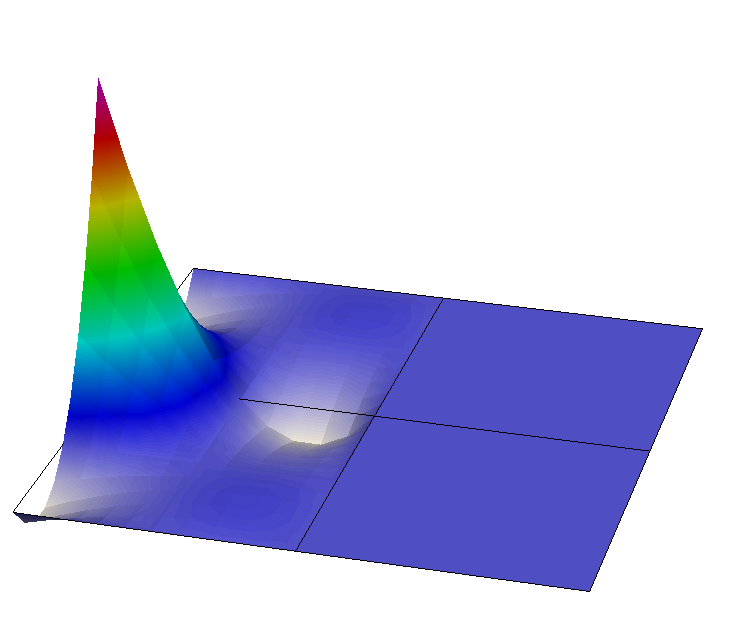
\includegraphics[height=.20\textwidth]{graph/cgbasis1-02}
    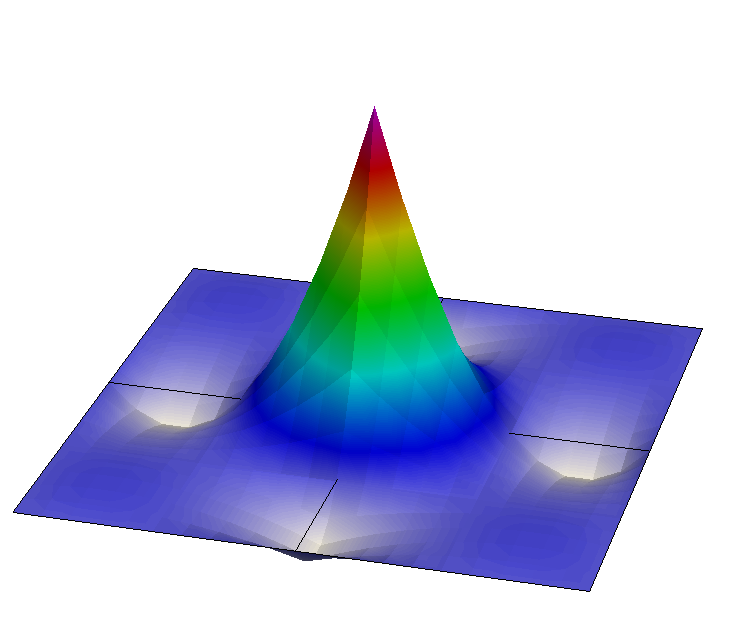
\includegraphics[height=.20\textwidth]{graph/cgbasis1-03}
    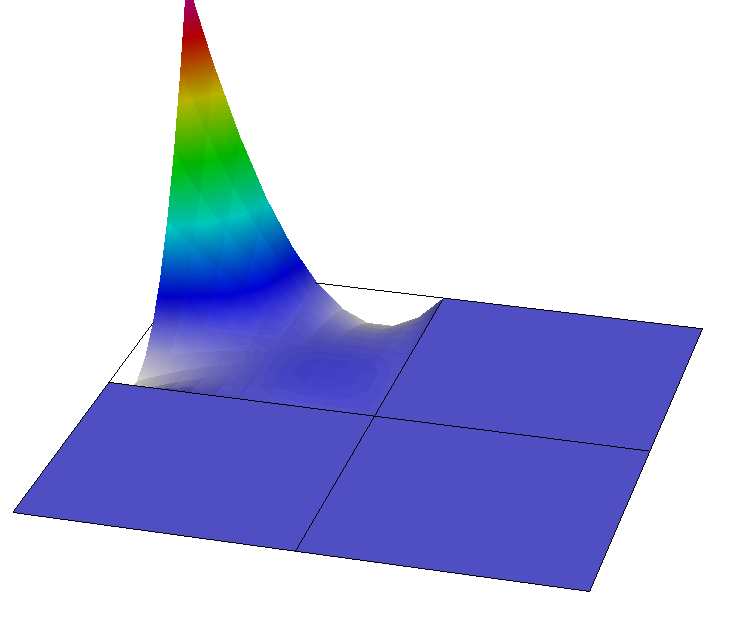
\includegraphics[height=.20\textwidth]{graph/cgbasis1-15}
    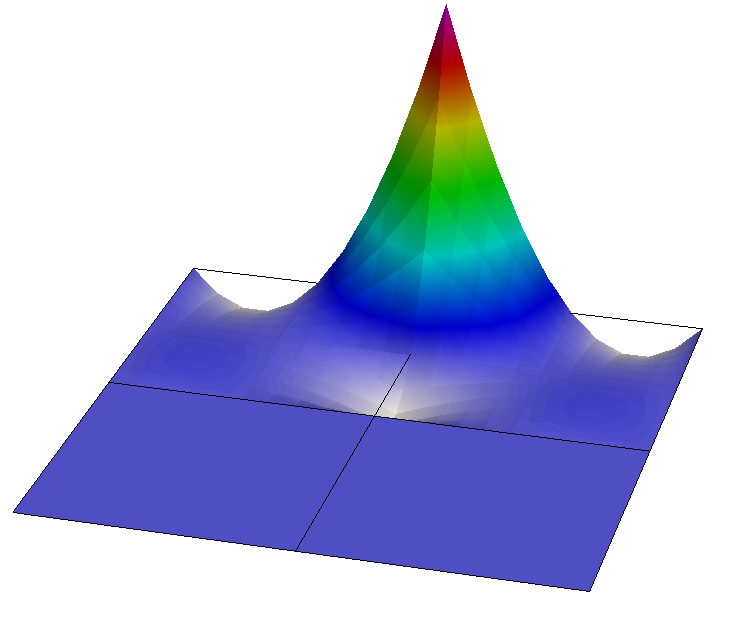
\includegraphics[height=.20\textwidth]{graph/cgbasis1-16}

    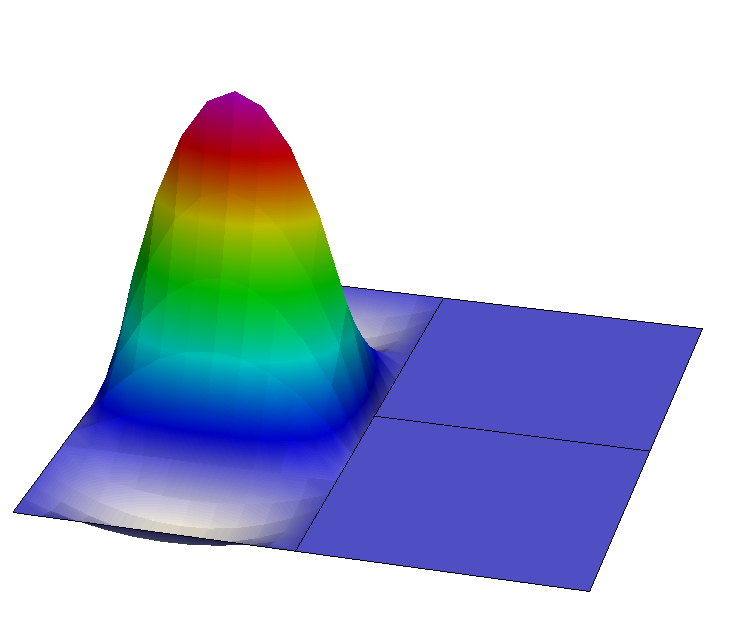
\includegraphics[height=.20\textwidth]{graph/cgbasis1-07}
    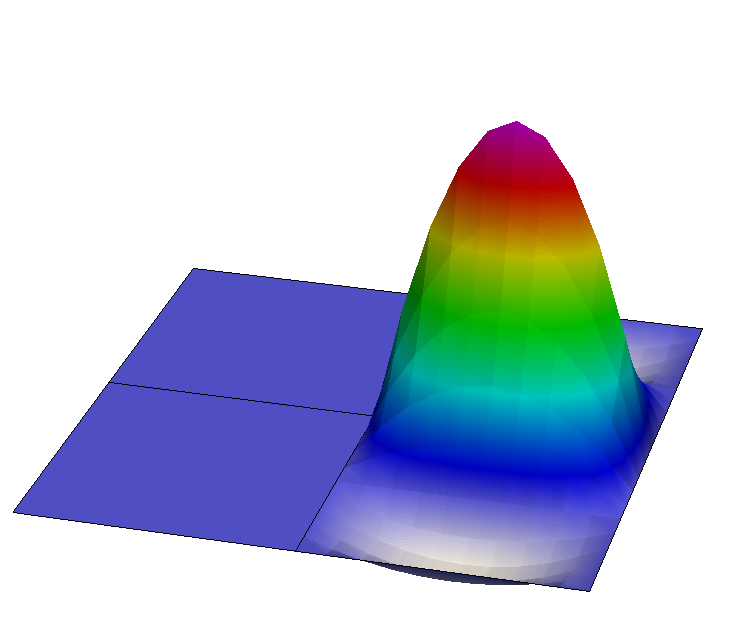
\includegraphics[height=.20\textwidth]{graph/cgbasis1-13}
    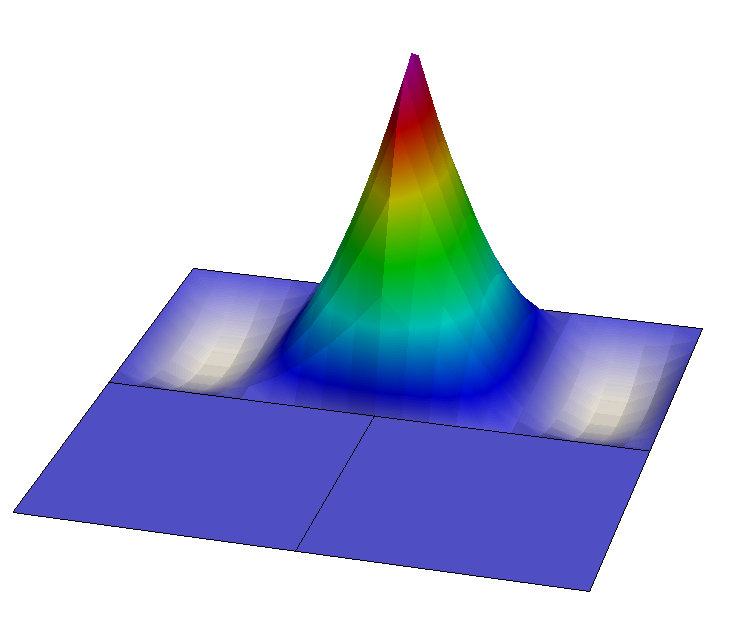
\includegraphics[height=.20\textwidth]{graph/cgbasis1-18}
    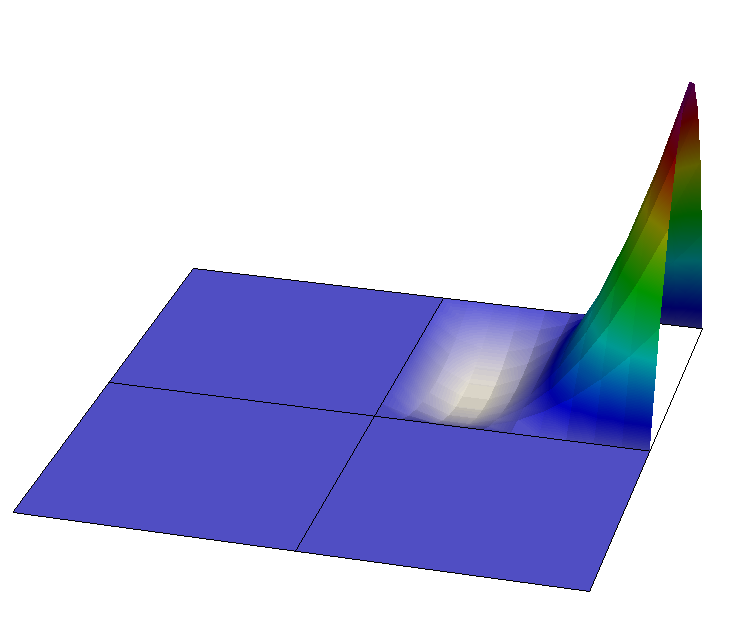
\includegraphics[height=.20\textwidth]{graph/cgbasis1-22}

    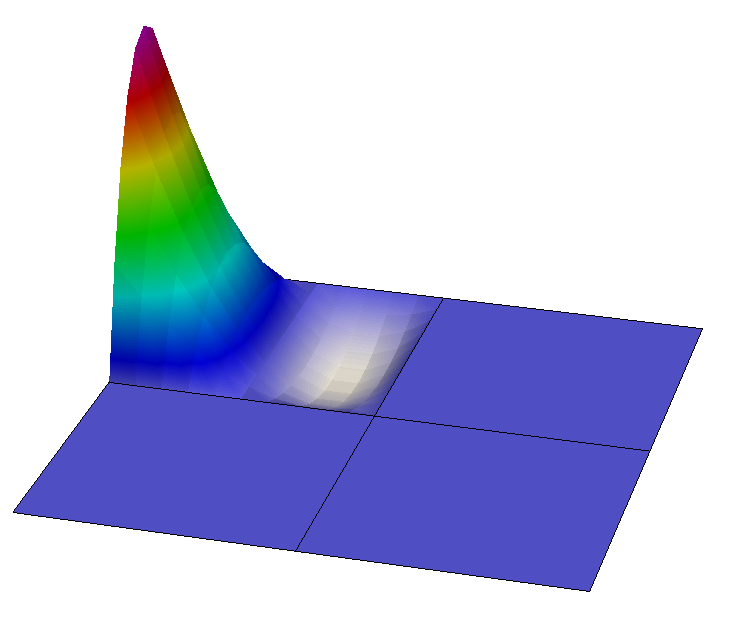
\includegraphics[height=.20\textwidth]{graph/cgbasis1-17}
    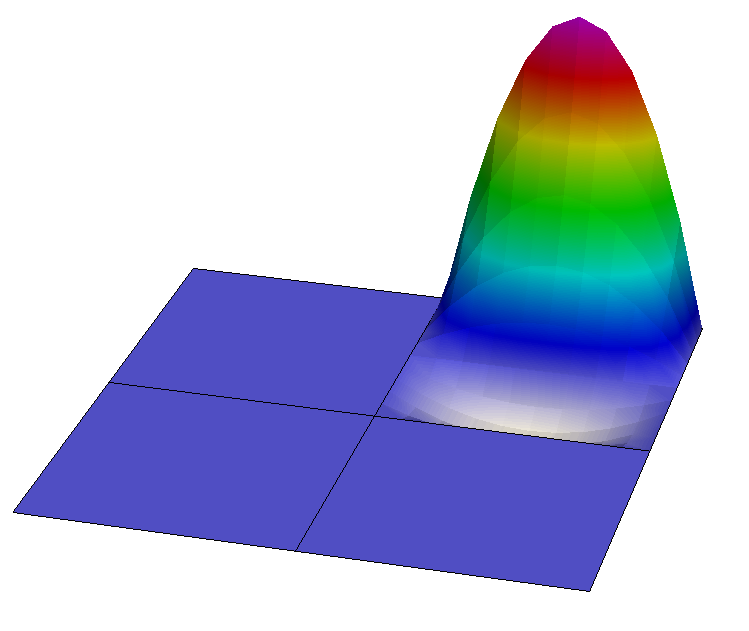
\includegraphics[height=.20\textwidth]{graph/cgbasis1-23}
    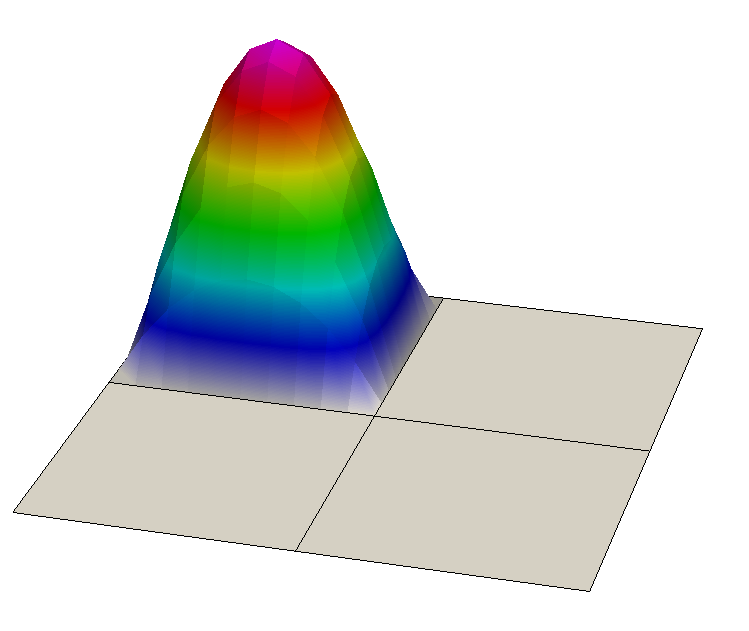
\includegraphics[height=.20\textwidth]{graph/cgbasis1-20}
    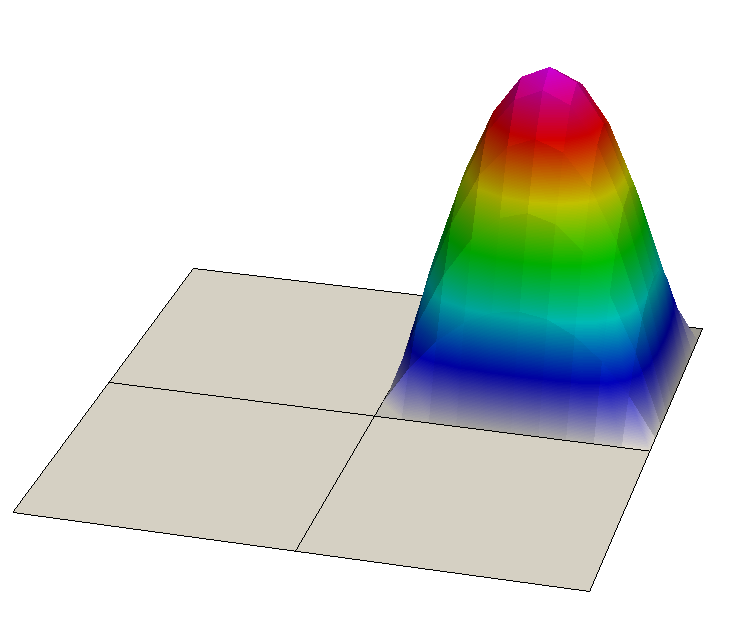
\includegraphics[height=.20\textwidth]{graph/cgbasis1-24}
  \end{center}
\end{Example*}

\begin{Example*}{dg-q2}{Discontinuous basis functions}
  \begin{center}
    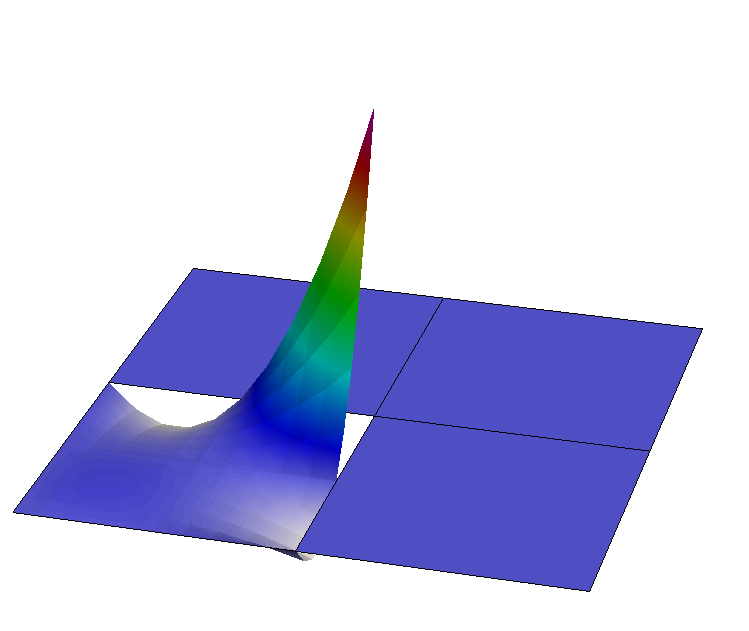
\includegraphics[height=.20\textwidth]{graph/dgbasis1-08}
    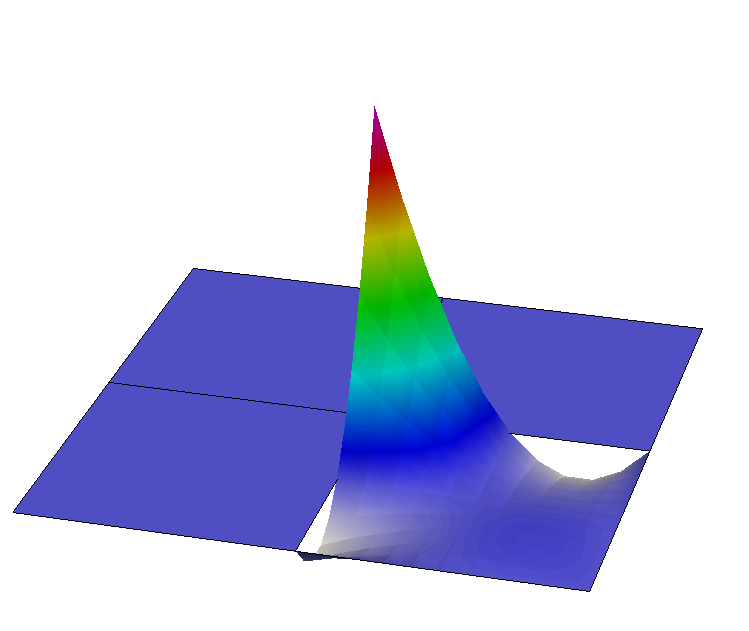
\includegraphics[height=.20\textwidth]{graph/dgbasis1-15}
    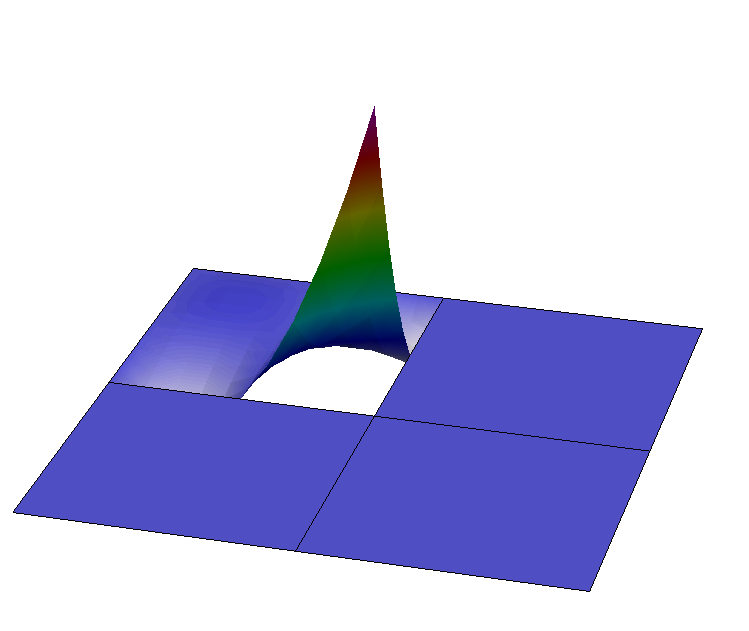
\includegraphics[height=.20\textwidth]{graph/dgbasis1-20}
    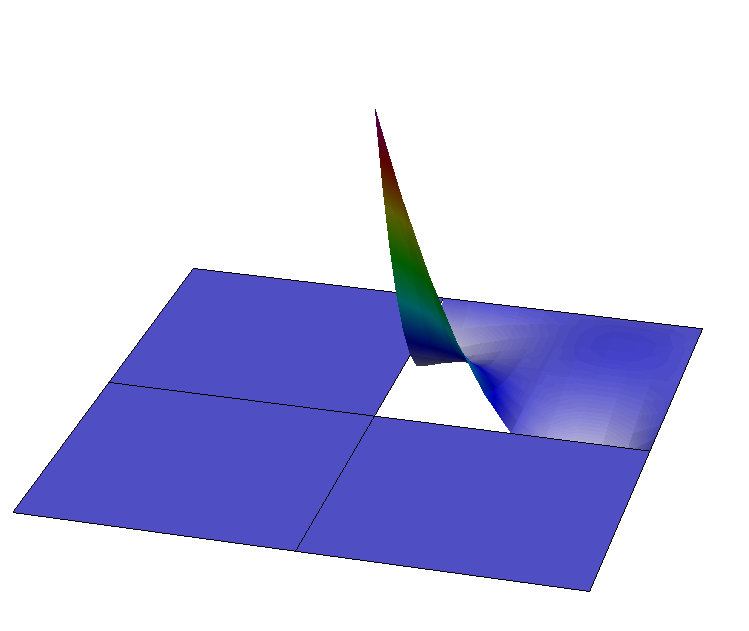
\includegraphics[height=.20\textwidth]{graph/dgbasis1-27}

    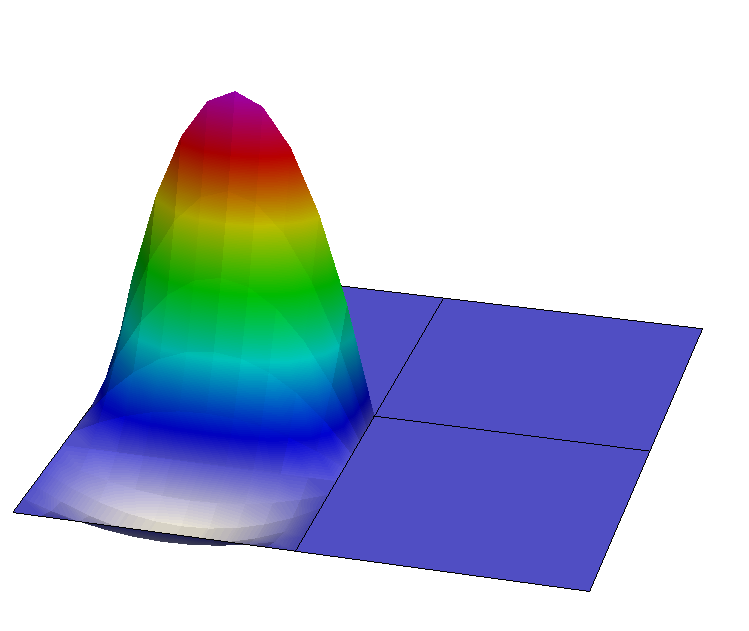
\includegraphics[height=.20\textwidth]{graph/dgbasis1-07}
    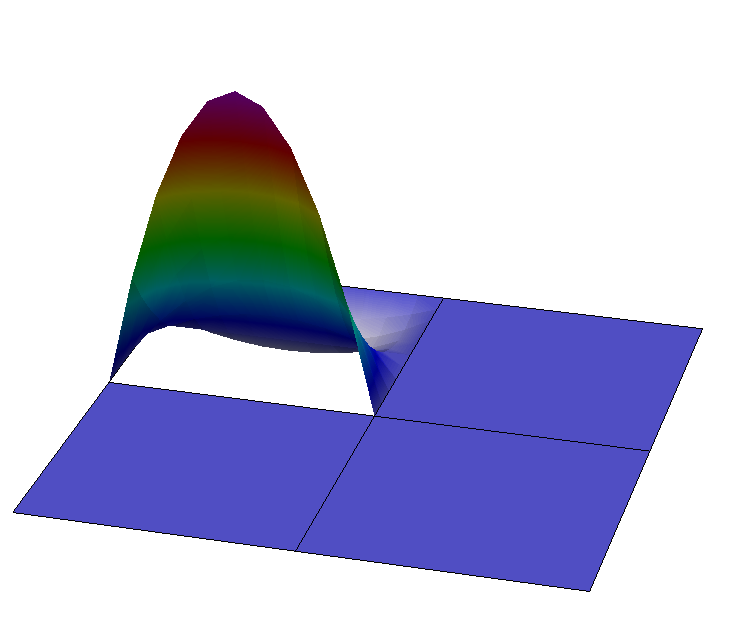
\includegraphics[height=.20\textwidth]{graph/dgbasis1-19}
    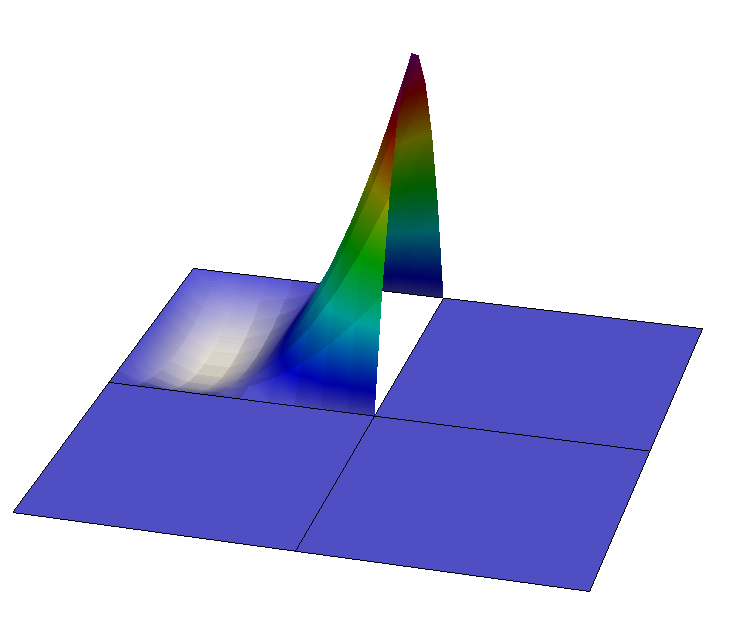
\includegraphics[height=.20\textwidth]{graph/dgbasis1-23}
    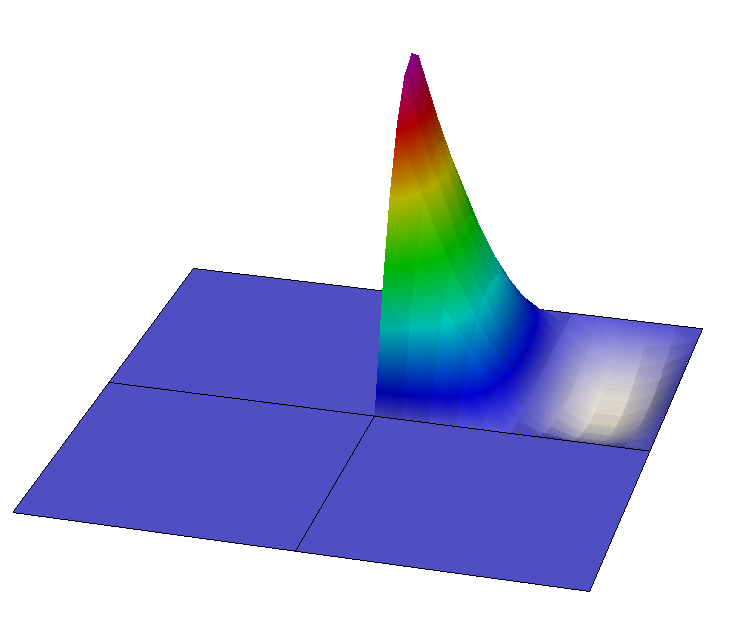
\includegraphics[height=.20\textwidth]{graph/dgbasis1-30}

    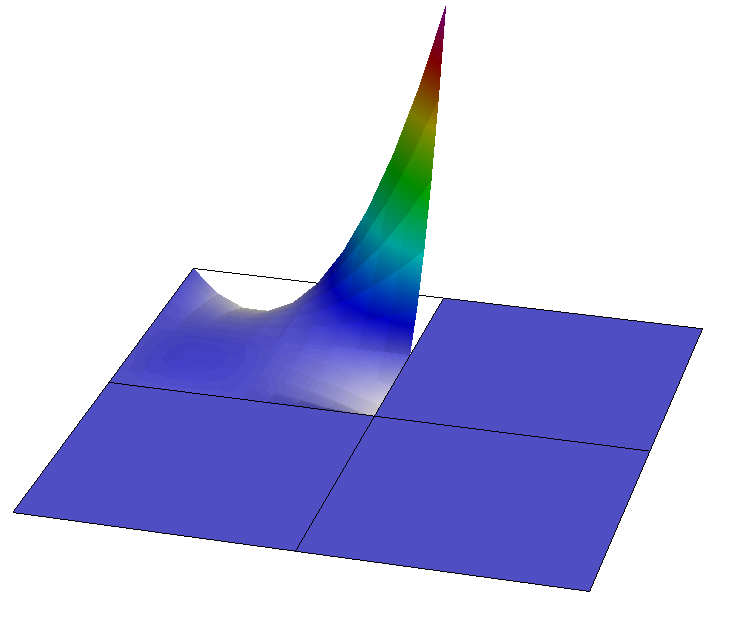
\includegraphics[height=.20\textwidth]{graph/dgbasis1-26}
    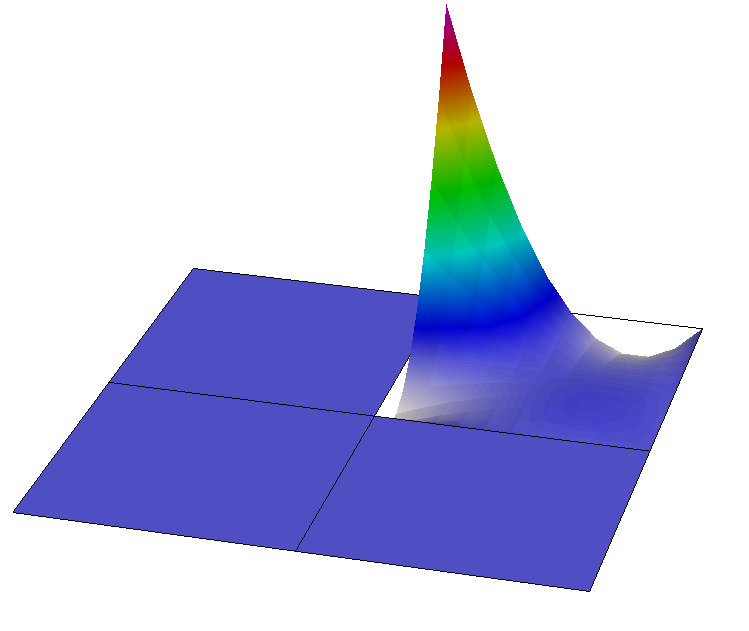
\includegraphics[height=.20\textwidth]{graph/dgbasis1-33}
    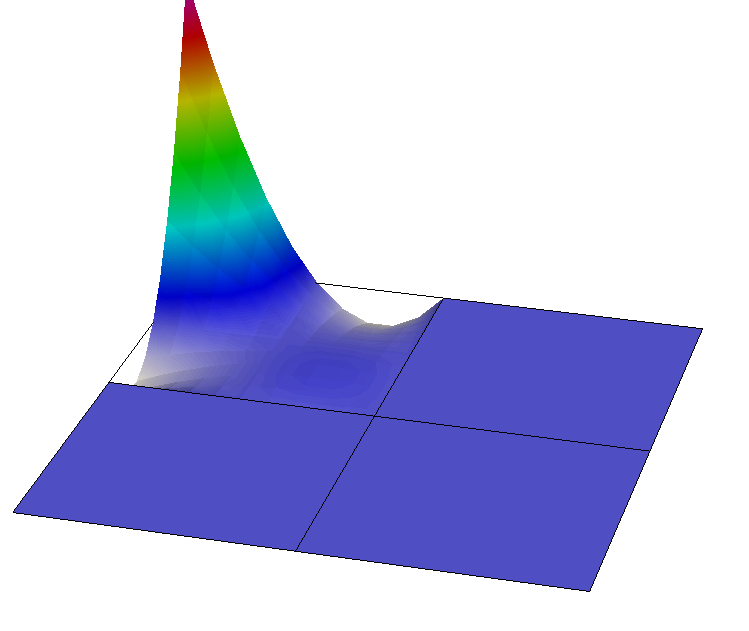
\includegraphics[height=.20\textwidth]{graph/dgbasis1-24}
    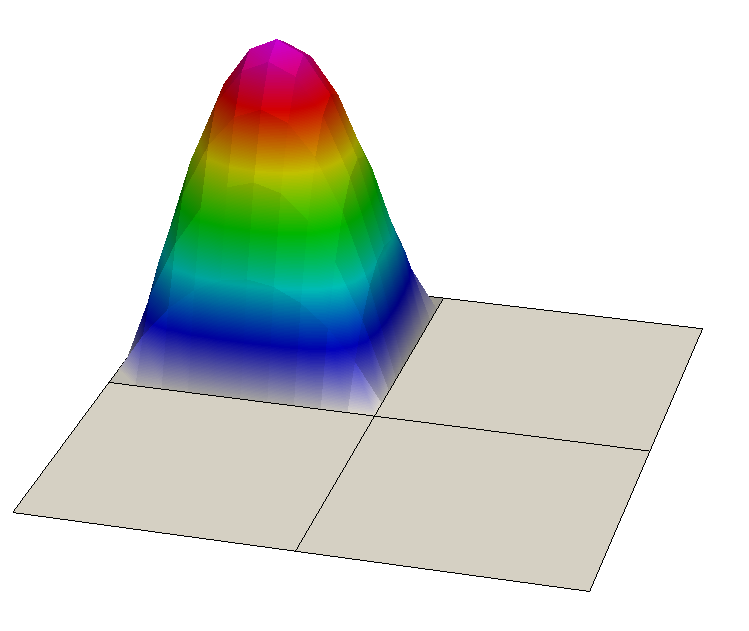
\includegraphics[height=.20\textwidth]{graph/dgbasis1-22}
  \end{center}
\end{Example*}

\begin{example}
  As a second example, we choose $d=2$ and the univariate space $\P_2$ with node functionals
  \begin{gather}
    \nodal_0(p) = p(0),
    \quad \nodal_1(p) = \int_0^1 p(t) \dt,
    \quad \nodal_2(p) = p(1),
  \end{gather}
  that is, a mixture of Lagrange interpolation and orthogonality on
  the interval $[0,1]$. The matching basis polynomials are
  \begin{gather}
    p_0(t) = 3(1-t)^2 - 2(1-t),
    \quad p_1(t) = 6 t(1-t),
    \quad p_2(t) = 3t^2-2t.
  \end{gather}
  Follwoing the construction of the previous example, we obtain
  \begin{gather}
    \begin{aligned}
    \nodal_{00}(p) &= p(0,0),
    &\nodal_{02}(p) &= p(0,1),\\
    \nodal_{20}(p) &= p(1,0),
    &\nodal_{22}(p) &= p(1,1).
    \end{aligned}
  \end{gather}
  Then,
  \begin{gather}
    \nodal_{01}(p_{01}) = \nodal_{01}(p_0\otimes p_1)
    = p_0(0)\int_0^1 p_1(y)\dy
    = \int_0^1 p(0,y) \dy.
  \end{gather}
  Thus, the node functional $\nodal_{01}$ is the integral over the
  left edge of the reference square. By the same construction,
  $\nodal_{01}$ is the integral over the right edge. $\nodal_{10}$ and
  $\nodal_{12}$ are the integrals over the bottom and top edge,
  respectively. Finally,
  \begin{gather}
    \nodal_{11}(p_{11})
    = \int_0^1 p_1(x)\dx \int_0^1 p_1(y) \dy
    = \int_0^1\int_0^1 p_{11}(x,y) \dx\dy.
  \end{gather}
  Thus, the tensor product of two line integrals becomes the integral
  over the area.
\end{example}



%%%%%%%%%%%%%%%%%%%%%%%%%%%%%%%%%%%%%%%%%%%%%%%%%%%%%%%%%%%%%%%%%%%%%%
%%%%%%%%%%%%%%%%%%%%%%%%%%%%%%%%%%%%%%%%%%%%%%%%%%%%%%%%%%%%%%%%%%%%%%
\subsection{The Galerkin equations and Céa's lemma}
%%%%%%%%%%%%%%%%%%%%%%%%%%%%%%%%%%%%%%%%%%%%%%%%%%%%%%%%%%%%%%%%%%%%%%
%%%%%%%%%%%%%%%%%%%%%%%%%%%%%%%%%%%%%%%%%%%%%%%%%%%%%%%%%%%%%%%%%%%%%%

\begin{Definition*}{galerkin-approximation}{Galerkin approximation}
  Let $u\in V$ be determined by the weak formulation
  \begin{gather*}
    a(u,v) = f(v) \qquad\forall v\in V,
  \end{gather*}
  where $V$ is a suitable function space including boundary
  conditions. The \define{Galerkin approximation}, also called
  \define{conforming approximation} of this problem reads as follows:
  choose a subspace $V_n\subset V$ of dimension $n$ and find
  $u_n\in V_n$, such that
  \begin{gather*}
    a(u_n,v_n) = f(v_n) \qquad\forall v_n\in V_n.
  \end{gather*}
  We will refer to this equation as the \define{discrete problem}.
\end{Definition*}

\begin{Corollary*}{galerkin-equations}{Galerkin equations}
  After choosing a basis $\{v_i\}$ for $V_n$, the Galerkin equations are
  equivalent to a linear system
  \begin{gather}
    \mata \vu = \vf,
  \end{gather}
  with $\mata\in\R^{n\times n}$ and $\vf\in \R^n$ defined by
  \begin{gather}
    a_{ij} = a(v_j, v_i), \qquad f_i = f(v_i).
  \end{gather}
\end{Corollary*}

\begin{Lemma}{discrete-lax-milgram}
  If the lemma of Lax-Milgram holds for $a(.,.)$ on $V$, it holds on
  $V_n\subset V$. In particular, solvability of the Galerkin equations
  is implied.
\end{Lemma}

\begin{Lemma*}{cea}{Céa}
  Let $a(.,.)$ be a bounded and elliptic bilinear form on the Hilbert
  space $V$. Let $u \in V$ and $u_n\in V_n$ be the solution to the
  weak formulation and its Galerkin approximation, respectively. Then,
  there holds
  \begin{gather}
    \norm{u-u_h}_V \le \frac{M}{\alpha}
    \inf_{v_n\in V_n}\norm{u-v_h}_V.
  \end{gather}
\end{Lemma*}

\begin{Lemma}{fe-matrix}
  For a finite element discretization of Poisson's equation with the
  space $V_\mesh$, the Galerkin equations can be computed using the
  following formulas:
  \begin{alignat*}3
    a_{ij} &= \int\limits_\domain \nabla v_j \cdot \nabla v_i \dx
    &&= \int\limits_{\domain(\nodal^i)} \nabla v_j \cdot \nabla v_i \dx
    &&= \sum_{\cell\in\mesh(\nodal^i)}\int\limits_\cell \nabla v_j \cdot \nabla v_i \dx\\
    f_{i} &= \int\limits_\domain f v_i \dx
    &&= \int\limits_{\domain(\nodal^i)} f v_i \dx
    &&= \sum_{\cell\in\mesh(\nodal^i)}\int\limits_\cell f v_i \dx
  \end{alignat*}
\end{Lemma}

\begin{Algorithm*}{matrix-assembling}{Assembling the matrix}
  \begin{enumerate}
  \item Start with a matrix $\mata = 0 \in \R^{n\times n}$
  \item Loop over all cells $\cell\in\mesh$
  \item On each cell $\cell$, compute a cell matrix
    $\mata_\cell \in \R^{n_\cell\times n_\cell}$ by integrating
    \begin{gather}
      a_{\cell,ij} = \int_\cell \nabla p_{\cell,j}\cdot\nabla p_{\cell,i}\,dx,
    \end{gather}
    where $\{p_{\cell,i}\}$ is the shape function basis.
  \item Assemble the cell matrices into the global matrix by
    \begin{gather}
      a_{\iota(i),\iota(j)} = a_{\iota(i),\iota(j)} + a_{\cell,ij}
      \qquad i,j = 1,\dots,n_\cell.
    \end{gather}
  \end{enumerate}
\end{Algorithm*}

%%%%%%%%%%%%%%%%%%%%%%%%%%%%%%%%%%%%%%%%%%%%%%%%%%%%%%%%%%%%%%%%%%%%%%
%%%%%%%%%%%%%%%%%%%%%%%%%%%%%%%%%%%%%%%%%%%%%%%%%%%%%%%%%%%%%%%%%%%%%%
\subsection{Mapped finite elements}
%%%%%%%%%%%%%%%%%%%%%%%%%%%%%%%%%%%%%%%%%%%%%%%%%%%%%%%%%%%%%%%%%%%%%%
%%%%%%%%%%%%%%%%%%%%%%%%%%%%%%%%%%%%%%%%%%%%%%%%%%%%%%%%%%%%%%%%%%%%%%

\begin{Definition}{mapped-mesh}
  A mapped mesh $\mesh$ is a set of cells $\cell$, which are defined
  by a single \define{reference cell} $\refcell$ and individual
  smooth mappings
  \begin{gather}
    \begin{split}
      \Phi_\cell \colon \refcell &\to \R^d\\
      \Phi_\cell(\refcell) &= \cell.
    \end{split}
  \end{gather}
  The definition extends to small sets of reference cells, for
  instance for triangles and quadrilaterals.
\end{Definition}

\begin{Example}{mapping-linear}
  Let the reference triangle $\refcell$ be defined by
  \begin{gather}
    \refcell = \left\{
      \begin{pmatrix}
        \refx\\\refy
      \end{pmatrix}
      \middle|
      \refx,\refy >0, \refx+\refy < 1
    \right\}.
  \end{gather}
  Then, every cell $\cell$ spanned by the vertices $\vertex_0$,
  $\vertex_1$, and $\vertex_2$ is obtained by mapping $\refcell$ by
  the \putindex{affine mapping}
  \begin{gather}
    \Phi_\cell(\refvx) =
    \begin{pmatrix}
      X_1-X_0 & X_2 - X_0 \\ Y_1-Y_0 & Y_2 - Y_0
    \end{pmatrix}
    \begin{pmatrix}
      \refx \\ \refy
    \end{pmatrix}
    +
    \begin{pmatrix}
      X_0 \\ Y_0
    \end{pmatrix} =: \matb_\cell \refvx + \vb_\cell
  \end{gather}
\end{Example}

\begin{Example}{mapping-bilinear}
  The reference cell for a quadrilateral is the reference square
  $\refcell = (0,1)^2$. Every quadrilateral $\cell$ spanned by the
  vertices $\vertex_0$ to $\vertex_3$ is then obtained by the
  \putindex{bilinear mapping}
  \begin{gather}
    \Phi_\cell(\refvx)
    = \vertex_0 (1-\refx)(1-\refy)
    + \vertex_1 \refx(1-\refy)
    + \vertex_2 (1-\refx)\refy
    + \vertex_3 \refx\refy
  \end{gather}
\end{Example}

\begin{Definition}{mapped-fe}
  Mapped shape functions $\{p_i\}$ on a mesh cell $\cell$ are defined by a
  set of shape functions $\{\refp_i\}$ on the reference cell
  $\refcell$ through \define{pull-back}
  \begin{gather}
    \begin{split}
      p_i(\vx) &= \refp_i\left(\Phi^{-1}(\vx)\right) = \refp_i(\refvx),\\
      \nabla p_i(\vx) &= \nabla\Phi^{-T}(\refvx)\refgrad\refp_i(\refvx)
    \end{split}
  \end{gather}
\end{Definition}

\begin{Lemma}{mapped-norms-affine}
  Let $\refcell$ be the reference triangle and let $\cell$ be a
  triangular mesh cell with mapping
  $\vx = \Phi_\cell(\refvx) = \matb \refvx + \vb$. Let there hold
  $u(\vx) = \refu(\refvx)$. Then, $u\in H^k(\cell)$ if and only if
  $\refu\in H^k(\refcell)$ and we have with some constant $c$ the
  estimates
  \begin{gather}
    \begin{split}
      \snorm{\refu}_{k,\refcell}
      &\le c \norm{\matb}^k (\det \matb)^{-\nicefrac12}
      \snorm{u}_{k,\cell},\\
      \snorm{u}_{k,\cell}
      &\le c \norm{\matb^{-1}}^k (\det \matb)^{\nicefrac12}
      \snorm{\refu}_{k,\refcell}.
    \end{split}
  \end{gather}
\end{Lemma}

\begin{Lemma}{shape-regular-transformation}
  For a cell $\cell$, let $R$ be the radius of the circumscribed
  circle and $\rho$ the radius of the inscribed circle. Then,
  \begin{gather}
    \norm{\matb} \le c R, \qquad \norm{\matb^{-1}} \le c \rho^{-1}.
  \end{gather}
\end{Lemma}

\begin{Assumption}{mapping-decomposition}
  For more general mappings $\Phi\colon \refcell\to \cell$, we
  make the assumption, that they can be decomposed into three factors,
  \begin{gather}
    \Phi = \Phi_O \circ \Phi_S \circ \Phi_W,
  \end{gather}
  where $\Phi_O$ is a combination of translation and rotation,
  $\Phi_S$ is a scaling with a characteristic length $h_T$, and
  $\Phi_W$ is a warping function not changing the characteristic length.
\end{Assumption}

\begin{example}
  We construct the inverse of $\Phi$ in two dimensions by the
  following three steps, using as $h_\cell$ the length of the longest
  edge of $\cell$.
  \begin{enumerate}
  \item Choose $\Phi_O$ as the rigid body movement which maps the
    longest edge to the interval $(0,h_\cell)$ on the $x$-axis and the
    cell itself to $\cell_O$ in the positive half plane. This mapping
    has the structure
    \begin{gather*}
      \Phi^{-1}_O (\vx) = \mats \vx - \mats \vertex_0,
    \end{gather*}
    where $\mats$ is an orthogonal matrix and $\vertex_0$ is the
    vertex moved to the origin.
  \item Choose the scaling
    \begin{gather*}
      \Phi^{-1}_S (\vx) = \tfrac1{h_\cell} \vx,
    \end{gather*}
    such that the longest edge of the resulting cell $\cell_S$ has the
    longest edge equal to the interval $(0,1)$ on the $x$-axis.
  \item Warp the cell $\cell_S$ into the reference cell $\refcell$ by
    the mapping $\Phi^{-1}_W$. This operation leaves the longest edge
    untouched. For triangles, it is the uniquely defined linear
    transformation mapping the vertex not on the longest edge to
    $(0,1)$. For quadrilaterals, it is a bilinear transformation.
  \end{enumerate}

  In the first step, we have assumed that the cell is convex, which is
  always true for triangles. For nonconvex quadrilaterals, it can be
  shown that the determinant of $\nabla\Phi$ changes sign inside the
  cell, such that these cells are not useful for computations.

  The idea of this decomposition is, that we separate mappings
  changing the position, size, and shape of the cells.
\end{example}

\begin{Lemma}{scaling-1}
  Let the typical length of a cell $\cell$ be $h_\cell$. Assume there
  are constants $0 < M_\cell, m_\cell, d_\cell, D_\cell$, such that
  \begin{gather}
    \begin{split}
      \norm{\nabla\Phi_W(\refvx)} \le M_\cell,
      \\
      \norm{\nabla\Phi_W^{-1}(\refvx)} \le m_\cell^{-1} ,
      \\
      d^2_\cell \le \det \nabla\Phi_W(\refx)) \le D^2_\cell.      
    \end{split}
  \end{gather}
  for all $\refvx\in\refcell$. Then, for $k=0,1$ and a constant $c$
  \begin{gather}
    \begin{split}
      \snorm{\refu}_{k,\refcell}
      &\le c \frac{M_\cell}{d_\cell}  h_\cell^{k-\nicefrac d2}
      \snorm{u}_{k,\cell},\\
      \snorm{u}_{k,\cell}
      &\le c \frac{D_\cell}{m_\cell} h_\cell^{\nicefrac d2-k}
      \snorm{\refu}_{k,\refcell}.
    \end{split}
  \end{gather}
  This extends to higher derivatives under assumptions on higher
  derivatives of $\Phi_\cell$.
\end{Lemma}

\begin{proof}
  By the chain rule,
  $\nabla \Phi_T = \nabla \Phi_O \nabla \Phi_S \nabla \Phi_W$. By
  construction, $\nabla\Phi_O$ is an orthogonal matrix, such that
  \begin{gather*}
    \norm{\nabla\Phi_O} = \norm{\nabla\Phi_O^{-1}} = 1.
  \end{gather*}
  Since it preserves angles and lengths, $\det \nabla\Phi_O =
  1$. Since $\Phi_S$ is a multiple of the identity, we have
  \begin{gather*}
    \norm{\nabla\Phi_S} = h_\cell,
    \quad\norm{\nabla\Phi_S^{-1}} = \frac1{h_\cell},
    \quad\det\nabla\Phi_S = h_\cell^d.
  \end{gather*}
  By change of variables, we have
  \begin{gather*}
    \int_\cell u^2 \dvx
    = \int_{\refcell} \refu^2 \abs{\det\nabla\Phi_\cell} \dvxref
    = \int_{\refcell} \refu^2 \det\nabla\Phi_S\det\nabla\Phi_O\det\nabla\Phi_W \dvxref
    ,
  \end{gather*}
  such that the case $k=0$ is proven immediately by
  \begin{gather*}
    h_T^d d_\cell^2 \int_{\refcell} \refu^2 \dvxref
    \le \int_\cell u^2 \dvx
    \le h_T^d D_\cell^2 \int_{\refcell} \refu^2 \dvxref
  \end{gather*}
  By the chain rule, we have
  \begin{gather*}
    \refgrad\refu(\refvx) = \nabla\Phi^T \nabla u(\vx)
    = \nabla\Phi_W^T \nabla\Phi_S^T \nabla\Phi_O^T \nabla u(\vx),
  \end{gather*}
  such that there holds
  \begin{gather}
    \begin{split}
      \abs{\refgrad\refu(\refvx)}
      &\le \norm{\nabla\Phi_W} h_\cell \abs{\nabla u},\\
      \abs{\nabla u(\vx)}
      &\le \norm{\nabla\Phi_W^{-1}} h_\cell^{-1} \abs{\refgrad \refu}.
    \end{split}
  \end{gather}
\end{proof}


\begin{Remark}{simple-mappings}
  We have $d_\cell = D_\cell$, if and only if the mapping is
  affine. The quotient $M_\cell/m_\cell$ measures how much the shape
  of the mesh cell deviates from the reference cell. For instance, it
  is one for squares.
\end{Remark}

%%% Local Variables: 
%%% mode: latex
%%% TeX-master: "main"
%%% End: 
